
\begin{figure}[h]
	\centering
	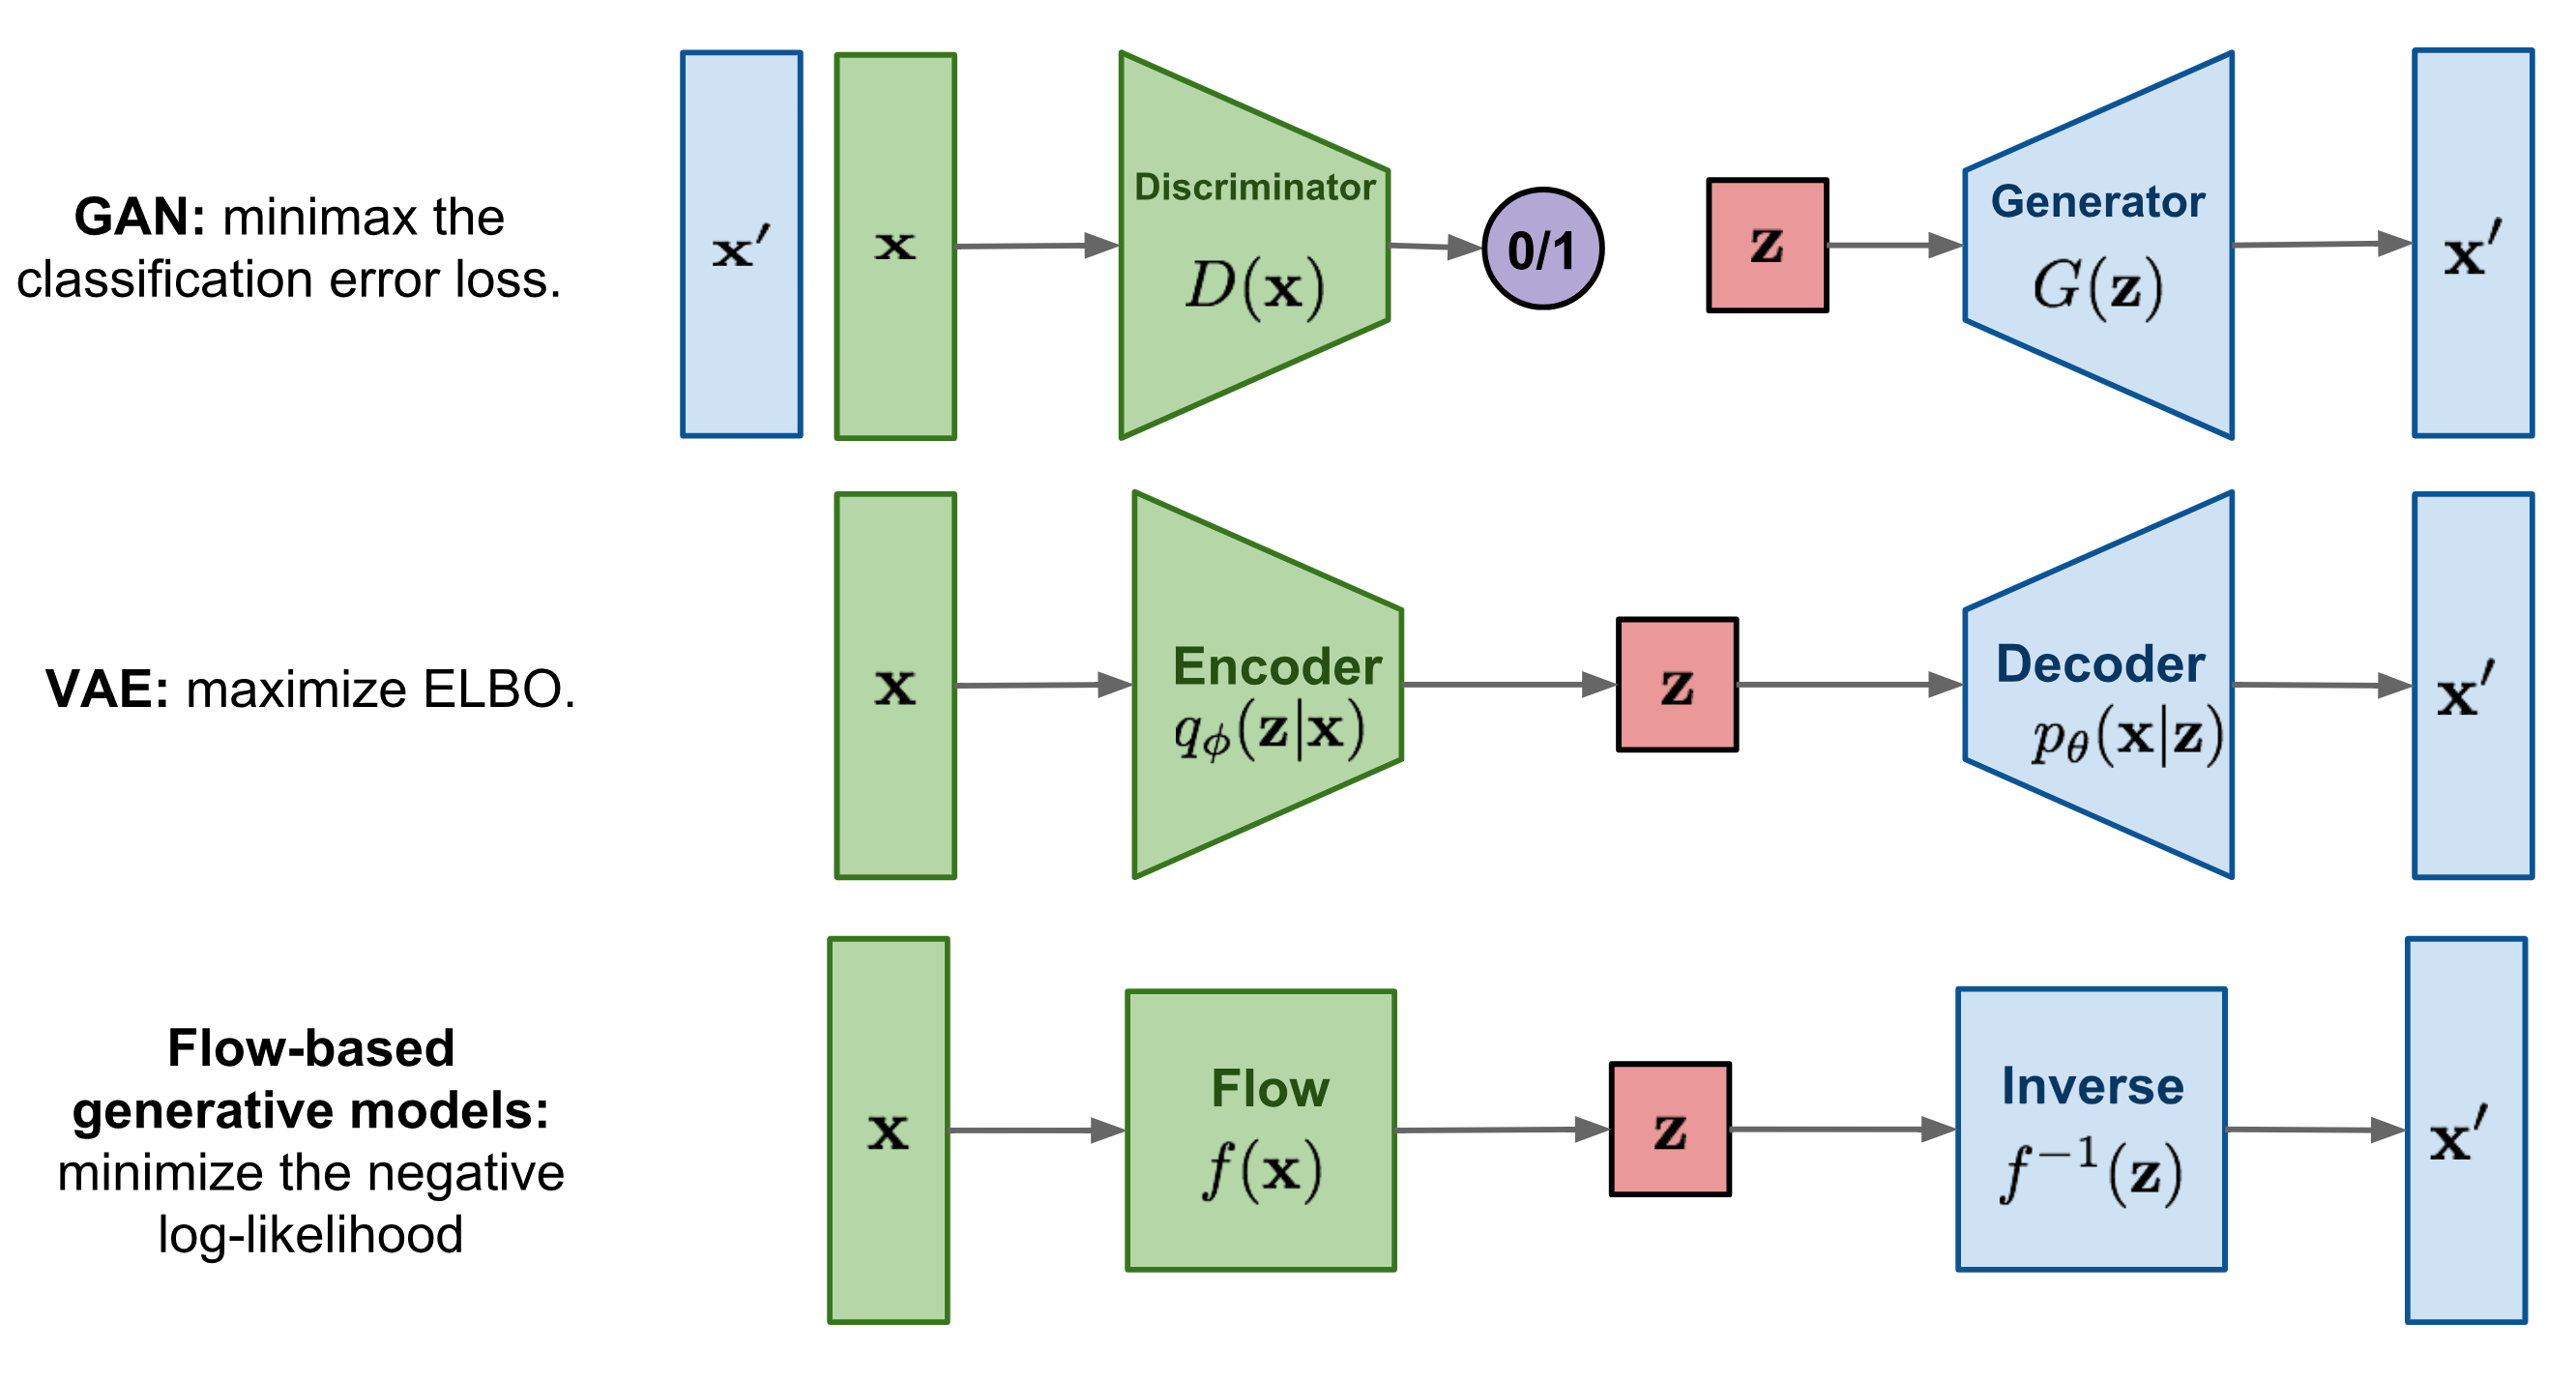
\includegraphics[scale=0.53]{./images/generative/flows/generative_models.png}
	\caption{An overview of generative models.}
\end{figure}

\begin{itemize}
	\item Flow-models get an exact estimate of the likelihood of your sample, as well as in the reverse direction. 
	\item VAEs optimize a lower bound on the (log) likelihood 
	\item GANs minimize a discrepancy between your input and transformed noise distributions. 
\end{itemize}



\section{The Method of Transformations of Random Variables}

If we are interested in finding the PDF of $Y=g(X)$, where $g(\cdot)$ is some deterministic transformation of $X$, and the function $g$ satisfies following properties, we can utilize a method called the method of transformations.
\begin{itemize}
	\item $g(x)$ is differentiable;
	\item $g(x)$ is a strictly (or monotonically) increasing function, that is, if $x_1<x_2$, then $g(x_1)<g(x_2)$.
\end{itemize}

% Now, let $X$ be a continuous random variable and $Y=g(X)$. We will show that you can directly find the PDF of $Y$ using the following formula.
% \begin{equation*}
% 	f_Y(y) = 
% 	\begin{cases}
% 	\frac{f_X(x_1)}{g'(x_1)}=f_X(x_1). \frac{dx_1}{dy} & \quad \textrm{where } g(x_1)=y\\
% 	0 & \quad \textrm{if }g(x)=y \textrm{ does not have a solution}
% 	\end{cases} 
% \end{equation*}

% Note that the derivative $\frac{dx}{dy}$ or $\frac{d}{dy}(g^{-1}(y))$ \textbf{measures how $X$ changes with respect to $Y$}.
% % Note that start with the function $y=f^{-1}(x)$. Write this as $x=f(y)$ and differentiate both sides implicitly with respect to$x$ using the Chain Rule:
% % \begin{align*}
% % 	1 &= f'(y)\frac{dy}{dx}\\
% % 	\frac{dy}{dx} &= \frac{1}{f'(y)}\\
% % 	y &= f^{-1}(x)\\
% % 	[f^{-1}]'(x) &= \frac{1}{f'(f^{-1}(x))}
% % \end{align*}
% Since $g$ is strictly increasing, its inverse function $g^{-1}$ is well defined. You can imagine a simple function like a linear function, \eg $Y=3X+1$. Then, for each $y\in R_Y$, there exists a \textbf{unique} $x_1$ such that $g(x_1)=y$. We can write $x_1=g^{-1}(y)$. Then,
% \begin{align*}
% 	\{Y\leq y\} = \{g(X)\leq y\} = \{X \leq g^{-1}(x)\}.
% \end{align*}
% Thus, 
% \begin{align*}
% 	F_Y(y) &= P(Y\leq y)\\
% 		   &= P(g(X)\leq y)\\
% 		   &= P(X\leq g^{-1}(y))\quad \text{, since }g \text{ is strictly increasing.}\\
% 		   &= F_X(g^{-1}(y)).
% \end{align*}
% To find the PDF of $Y$, we differentiate $F_Y(y)$ as follows:
% \begin{align*}
% 	f_Y(y) &= \frac{d}{dy}F_X(x_1)\quad \text{by } g(x_1)=y\\
% 		   &=\frac{dx_1}{dy}\cdot \underbrace{\frac{d}{dx_1}F_X(x_1)}_{=F'_X(x_1)}\\
% 		   &=\frac{dx_1}{dy}f_X(x_1)\\
% 		   &=f_X(g^{-1}(y))\left|\frac{d}{dy}(g^{-1}(y))\right|
% 		   % &= \frac{f_X(x_1)}{g'(x_1)} \quad \text{, since } \frac{dx}{dy}=\frac{1}{\frac{dy}{dx}}.
% \end{align*}
% We can repeat the same argument for the case where $g$ is \textbf{strictly decreasing}. In that case, $g'(x_1)$ will be \textbf{negative}, so we need to use $|g'(x_1)|$ . Thus, we can state the following theorem for a \textit{strictly monotonic function}. (A function $g:R\to R$ is called strictly monotonic if it is strictly increasing or strictly decreasing.)

% Actually, we assumed that $g$ was one-to-one out of convenience: the condition that $g$ is one-to-one is not necessary for change of variables to work: Consider a continuous random variable $X$ with domain $R_X$, and let $Y=g(X)$. Suppose that we can partition $R_X$ into a finite number of intervals such that $g(x)$ is strictly monotone and differentiable on each partition. Then the PDF of $Y$ is given by 
% \begin{align*}
% 	f_Y(y)= \sum_{i=1}^{n} \frac{f_X(x_i)}{|g'(x_i)|}= \sum_{i=1}^{n} f_X(x_i).
% 	\left|\frac{dx_i}{dy}\right|,
% \end{align*}
% where $x_1,\dots,x_n$ are real solutions to $g(x)=y$.

% \subsection{Intuitive Explanation}
How to derive the PDF of the random variable $Y=g(X)$ when one knows the PDF of the random variable $X$? If $X$ is discrete, we can derive the pmf for $Y$ by simply summing up the probability mass for all the $x$'s such that $f(x)=y$. For a general function $g$, there is no direct formula to get the PDF of the random variable $Y=g(X)$ knowing $p(X)$. There is a formula in case when $h$ is a differentiable one-to-one mapping from the range (\ie the support) of $X$ to the range of $Y$.

Take for example a random variable $X\sim \mathcal{N}(\mu, \sigma)$ and set $Y=\exp(X)$. The figure below shows some simulations of $X$ and the corresponding values of $Y$. The density of $X$ is shown in blue and the one of $Y$ is shown in orange in the vertical direction.

\begin{figure}[t]
	\centering
	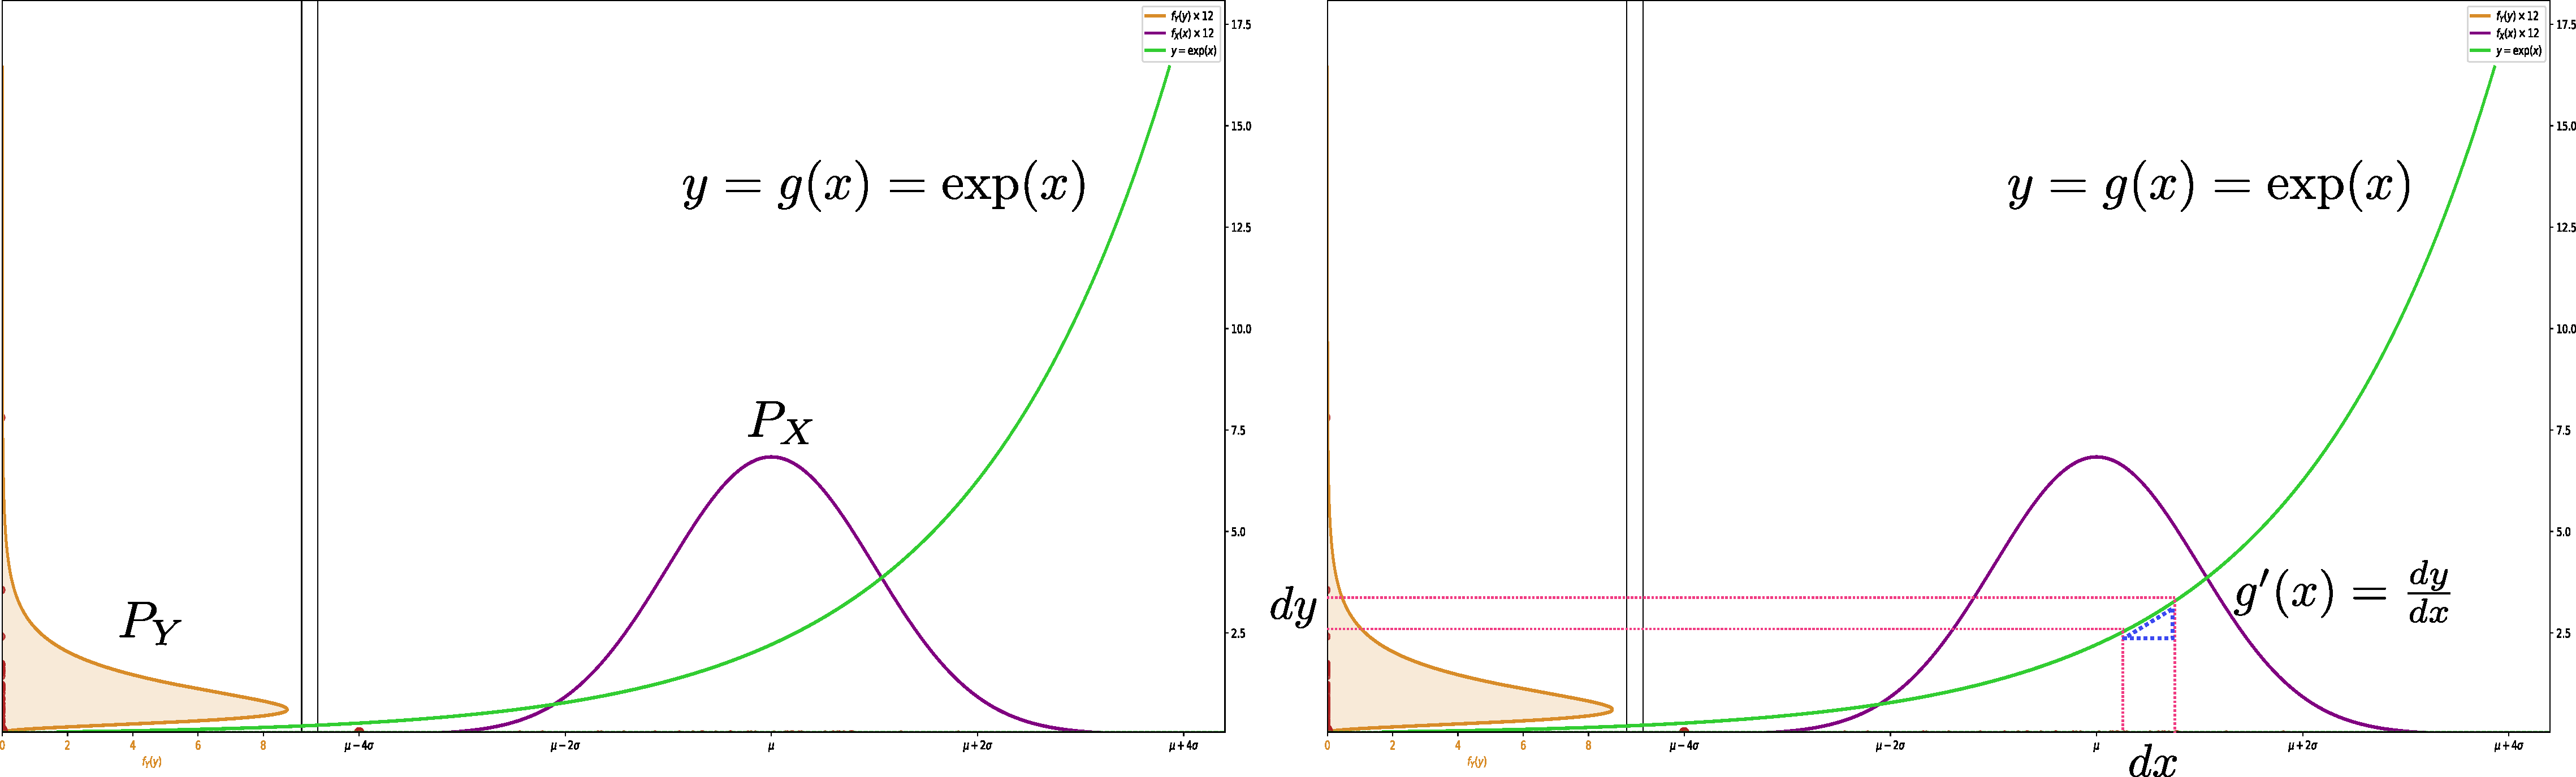
\includegraphics[scale=0.23]{./images/generative/flows/change_of_vars.pdf}
\end{figure}

\begin{figure}[t]
    \centering
    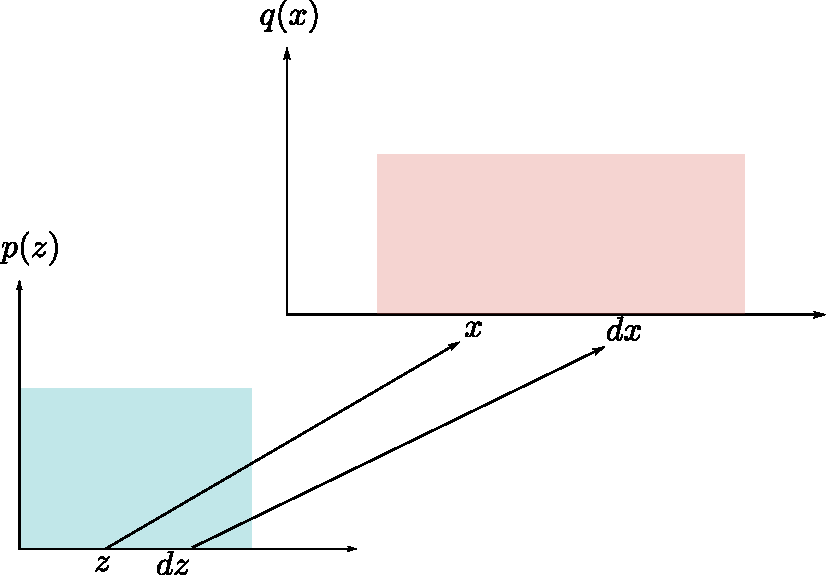
\includegraphics[scale=0.7]{./images/generative/flows/change_intuition.pdf}
    \caption{Area would be approximately $p(z)dz = q(z)dx$. Thus, $q(x) = p(z)\Big|\frac{dz}{dx}\Big|$}
    \label{fig:change_intuition}
\end{figure}


% \begin{figure}[ht]
%     \centering
%     \begin{minipage}[b]{0.45\textwidth}
%         \centering
%         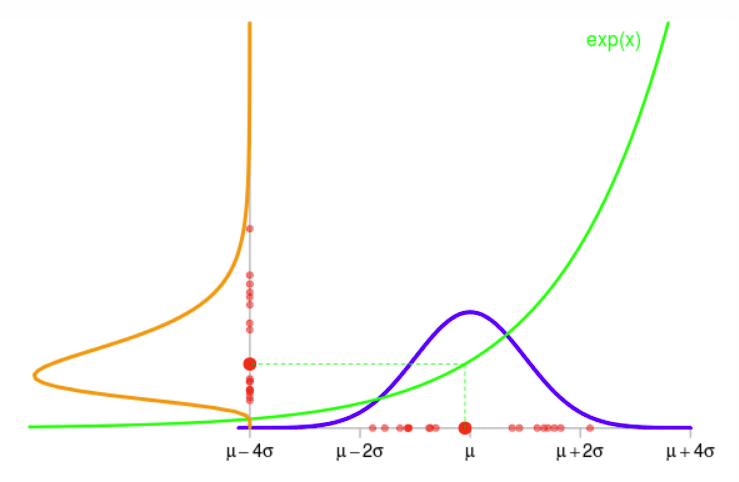
\includegraphics[width=\textwidth]{./images/generative/flows/sample.png}
%     \end{minipage}
%     \hfill
%     \begin{minipage}[b]{0.45\textwidth}
%         \centering
%         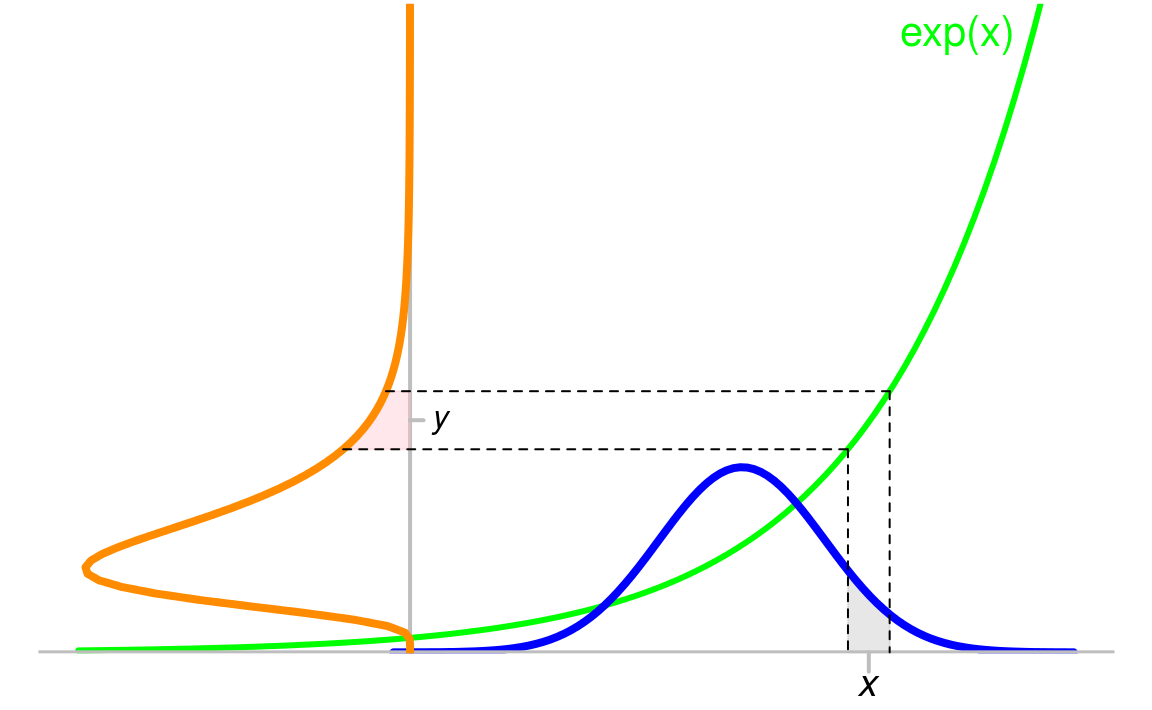
\includegraphics[width=\textwidth]{./images/generative/flows/sample2.png}
%     \end{minipage}
% \end{figure}
Now the question is: knowing the density of $X$, what is the density of $Y$?
Taking a point $y$ in the range of $Y$, the PDF $f_Y$ provides the probability of $Y$, belong to a small area $dy$ around $y$ by the formula below
$$P(Y\in dy)\approx f_Y(y)|dy|,$$
where $P(Y\in dy)$ is the area below the curve. Similarly, we can define
$$P(X\in dx)\approx f_X(x)|dx|$$
The above two areas are approximately the same in case of very small region. Note that if $dy$ and $dx$ are very small, we can approximate the derivative of $g'(x)=\frac{|dy|}{|dx|}$. Compactly, this can be expressed as follows:
$$P(X\in dx) = f_X(x)\frac{|dy|}{g'(x)}$$
With $y=g(x)$ we can get 
\begin{align*}
	P(X\in dx)\approx P(Y\in dy) &= f_X(x)\frac{|dy|}{g'(x)}\\
	& = f_X(g^{-1}(y))\frac{|dy|}{g'(g^{-1}(y))}\\
	& = f_X(g^{-1}(y))|dy|(g^{-1})'(y)
\end{align*}
The last line is by the derivative of inverse function which is 
$$\frac{d}{dx}f^{-1}(x) = \frac{1}{f'(f^{-1}(x))}$$
Finally, we can get 
$$f_Y(y) = f_X(g^{-1}(y))|(g^{-1})'(y)|$$
Note that the absolute is determined by the function $h$. This is the so-called \textit{change of variables formula}.



\subsection{Vector to Vector}

$Z$ and $X$ be random variables which are related by a mapping $f:\mathbb{R}^n\to \mathbb{R}^n$ such that $X=f(Z)$ and $Z=f^{-1}(X)$. Then
\begin{align*}
	p_X(\mathbf{x}) = p_Z(f^{-1}(\mathbf{x})) \left\vert \text{det}\left(\frac{\partial f^{-1}(\mathbf{x})}{\partial \mathbf{x}}\right) \right\vert
\end{align*}

Note that for any invertible square matrix $A$ over a field (\eg real or complex numbers),
\begin{align*}
	\det\bigl(A^{-1}\bigr)=\frac{1}{\det(A)}.
\end{align*}

Let
$$
A=\begin{bmatrix}
2 & 1\\[2pt]
3 & 4
\end{bmatrix}.
$$

Then, determinant of $A$ is given by
$$
\det(A)=2\cdot4-3\cdot1 = 8-3 = 5.
$$

The inverse of $A$ is 
$$
A^{-1}= \frac{1}{5}\begin{bmatrix}
4 & -1\\[2pt] -3 & 2
\end{bmatrix}.
$$

Then, the determinant of $A^{-1}$ is
$$
\det(A^{-1}) = \frac{1}{5^2}\bigl(4\cdot2-(-3)(-1)\bigr)
=\frac{1}{25}(8-3)=\frac{5}{25}=\frac{1}{5}.
$$

You can confirm the property:

$$
\det(A^{-1})=\frac{1}{5}=\frac{1}{\det(A)}.
$$


For example, we can transform $(x_1,x_2)$ to $(r,\theta)$ via $x_1=r\cos\theta$ and $x_2=r\sin\theta$.

Then
\[
J_{y\to x}=
\begin{pmatrix}
\dfrac{\partial x_1}{\partial r} & \dfrac{\partial x_1}{\partial\theta}\\[6pt]
\dfrac{\partial x_2}{\partial r} & \dfrac{\partial x_2}{\partial\theta}
\end{pmatrix}
=
\begin{pmatrix}
\cos\theta & -r\sin\theta\\
\sin\theta & \phantom{-}r\cos\theta
\end{pmatrix},
\tag{3}
\]
so
\[
\bigl|\det J_{y\to x}\bigr|
 = \bigl|\,r\cos^{2}\theta + r\sin^{2}\theta\,\bigr|
 = |r|.
\tag{4}
\]

Hence
\[
p_{\mathbf{y}}(\mathbf{y}) = p_{\mathbf{x}}(\mathbf{x})\,|J_{y\to x}|
\quad\Longrightarrow\quad
p_{R,\Theta}(r,\theta) = p_{X_1,X_2}(x_1,x_2)\,r.
\tag{5--6}
\]

For a two dimensional random vector $(X,Y)$ with density $p_{X,Y}$, 
\begin{align*}
	Pr((X,Y)\in A) = \int\int_A p_{X,Y}(x,y)dxdy.
\end{align*}
For a infinitesimally small region, we can approximate as follows:
\begin{align*}
	\int_x^{x+dx} p_{X}(x)dx \approx  p_{X}(x)dx.
\end{align*}

Similarly, we can get the probability as follows:
\[
P\!\bigl(r\le R\le r+dr,\;
        \theta\le\Theta\le\theta+d\theta\bigr)
  = p_{R,\Theta}(r,\theta)\,dr\,d\theta.
\tag{7}
\]
Note that the length of arc is $r\times d\theta$. Thus, the area $r\,dr\,d\theta$ or probability is given by
\[
P\!\bigl(r\le R\le r+dr,\;
        \theta\le\Theta\le\theta+d\theta\bigr)
  = p_{X,Y}(r\cos\theta, r\sin\theta)\,r\,dr\,d\theta,
\tag{8--9}
\]
so that finally
\[
p_{R,\Theta}(r,\theta)
  = p_{X,Y}(r\cos\theta, r\sin\theta)\,r.
\tag{10}
\]

% \begin{figure}[h]
%   \centering
%   % Replace the filename with the actual graphic if you have it.
%   \includegraphics[width=.55\linewidth]{polar_patch}
%   \caption{Change of variables from polar to Cartesian.
%            The area of the shaded patch is $r\,dr\,d\theta$.}
%   \label{fig:polarPatch}
% \end{figure}
